\documentclass{article}
\usepackage{graphicx}
\usepackage{xcolor}
\usepackage[document]{ragged2e}
\usepackage[a4paper, total={6in, 10in}]{geometry}
\author{Kulwinder Kaur (2021PHS7190), Harikesh Kushwaha (2021PHS7181)}
\title{\textbf{Extracting the Coordintes of the Center of a Drop from an Image}}
\date{}
\begin{document}
\maketitle
\hrule
\section*{A Brief Overview}
The goal of the article is to give a brief overview of the steps involved in extracting information about the center of a liquid drop from an image. The steps are as follows:\\
\textbf{0. Reading the Image:} Reads the image using \textcolor{orange}{matplotlib} to convert them into \textcolor{orange}{numpy arrays}.\\
\textbf{1. Cropping the Image:} Only a small portion of image is relevant to our analysis. To this end, the second step involves identifying the \textit{region of interest} and crop the image to include just that. \\
\textbf{2. Subtracting from a Reference Image:} The image contains a lot of \textit{noise} which can result in our method to fail while extracting the center of the drop. To overcome this, the third step involves subrating the image in consideration with a \textit{reference image} giving a "noise-less" image.\\
\textbf{3. Thresholding the Image:} This step converts the subtracted \textit{grayscale} image into a \textit{binary} one where all the pixels are either 0 or 1.\\
\textbf{4. Finding All Points on the "Circumference":} The step involves looping through both \textit{rows} and \textit{columns} of the image and finding the coordinates of all the \textit{pixels} with value 1 (corresponding to the white pixels). These points form the circumerference of the drop.\\
\textbf{5. Fitting an Ellipse to the Points:} In the final step, a generel ellipse is \textit{fitted} to the points found in step 4. The method uses the \textcolor{orange}{EllipseModel} \textit{class} from the \textcolor{orange}{skimage} \textit{library}. The class takes the X and Y coordinates of all thepoints and fits an ellipse using the \textit{least square} method. After fitting, the model returns the \textit{x and y coordinates} of the center of the ellipse, the \textit{semi major} and \textit{semi minor} axes and the angle $\mathit{\theta}$ between major axis and x axis.\\
\textbf{Please see the images below for a visual representation of the steps.}\\
\begin{flushleft}
  These steps are then repeated for all the images.
\end{flushleft}

% \begin{figure}
\centering
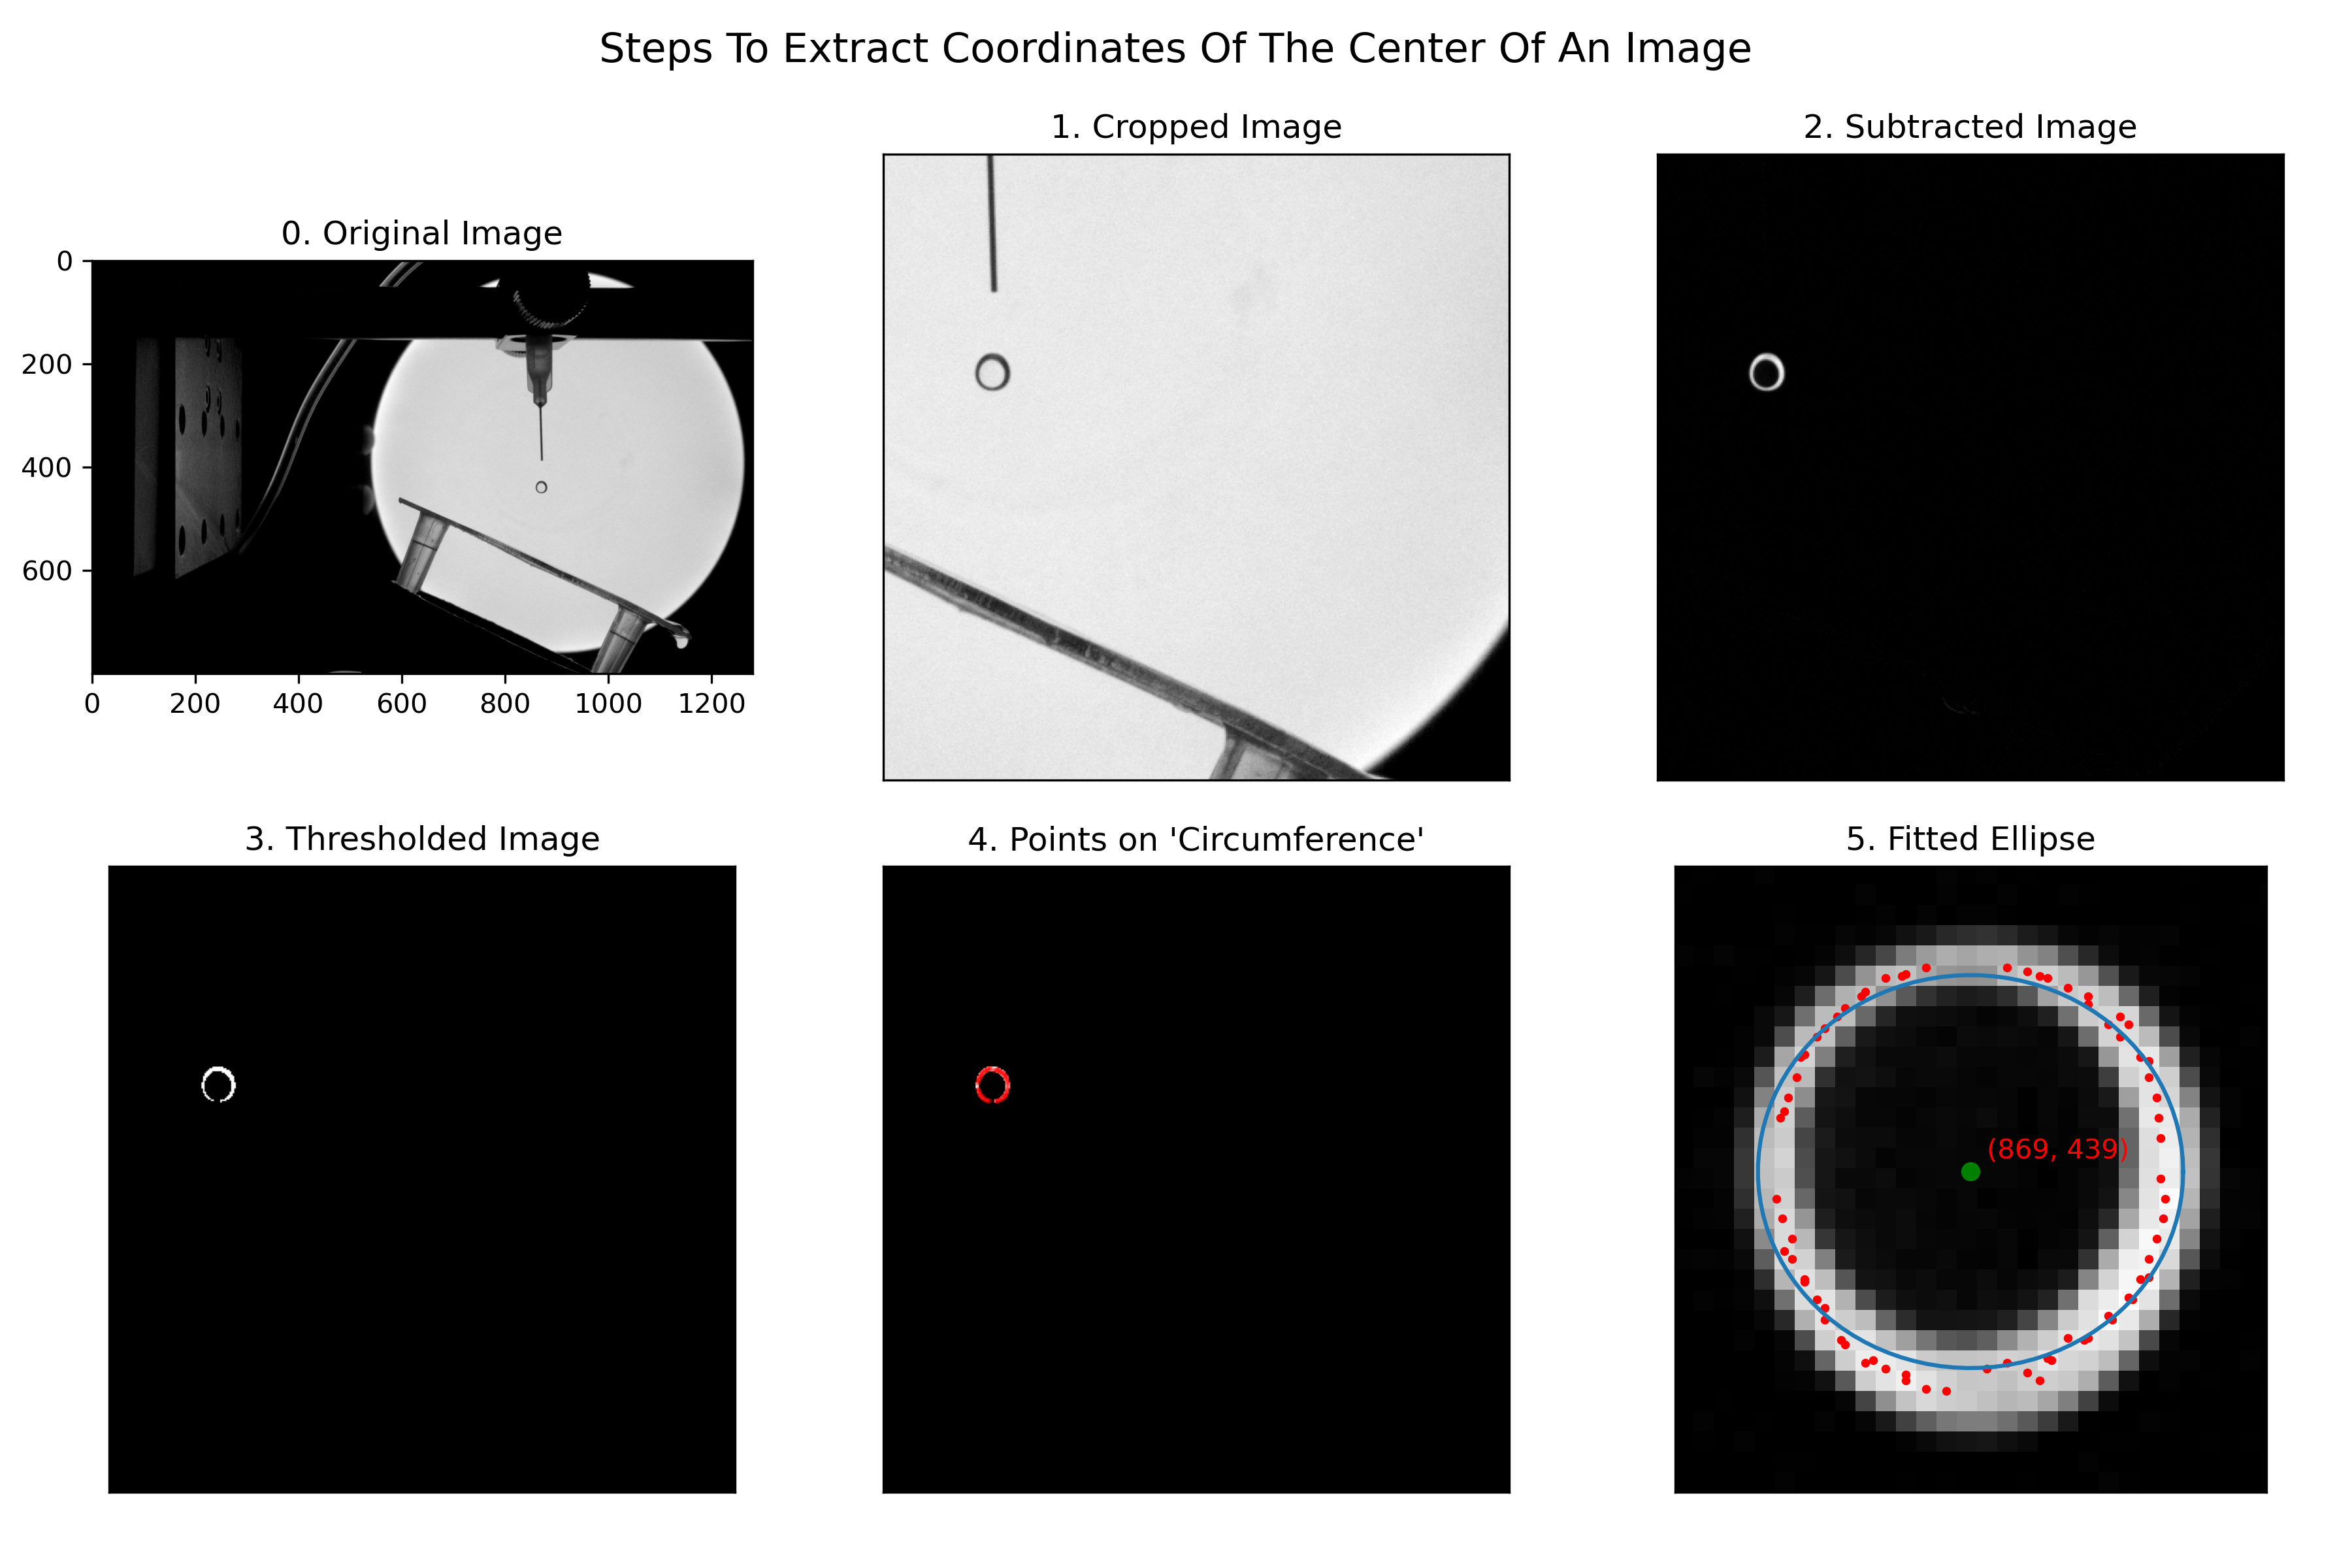
\includegraphics[scale=0.5]{final.png}
% \caption[]{Image Before and After Cropping and Thresholding}
% \end{figure}
\end{document}